\documentclass{standalone}

\usepackage{tikz}
\tikzset{>=latex}
\usetikzlibrary{arrows}

\begin{document}
        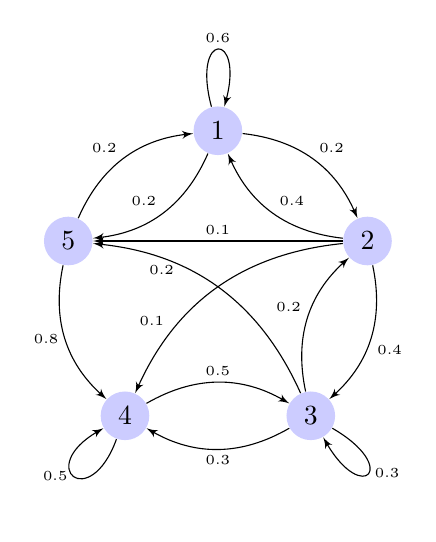
\begin{tikzpicture}[scale=2]
			\tikzset{edge/.style = {->,> = latex'}}
			\tikzset{point/.style = {circle,fill=blue!20}}

			\node[point] (n1) at (0,1) {1};
			\node[point] (n2) at (0.95, 0.3) {2};
			\node[point] (n3) at (0.59,-0.81) {3};
			\node[point] (n4) at (-0.59, -0.81) {4};
			\node[point] (n5) at (-0.95, 0.3) {5};
			
			\tiny
			
			\draw[edge] (n1) to[loop above] node[above, midway] {0.6} (n1);
			\draw[edge] (n1) to[bend left] node[above right, midway] {0.2} (n2);
			\draw[edge] (n1) to[bend left] node[above left, midway] {0.2} (n5);
			\draw[edge] (n2) to[bend left] node[above right, midway] {0.4} (n1);
			\draw[edge] (n2) to[bend left] node[below right, midway] {0.4} (n3);
			\draw[edge] (n2) to[bend right] node[above left, near end] {0.1} (n4);
			\draw[edge] (n2) to node[above, midway] {0.1} (n5);
			\draw[edge] (n3) to[in=-60,out=-30,loop] node[right] {0.3} (n3);
			\draw[edge] (n3) to[bend left] node[above left, midway] {0.2} (n2);
			\draw[edge] (n3) to[bend left] node[below, midway] {0.3} (n4);
			\draw[edge] (n3) to[bend right] node[below, near end] {0.2} (n5);
			\draw[edge] (n4) to[in=-150,out=-110, loop] node[left] {0.5} (n4);
			\draw[edge] (n4) to[bend left] node[above, midway] {0.5} (n3);
			\draw[edge] (n5) to[bend left] node[above left, midway] {0.2} (n1);
			\draw[edge] (n5) to[bend right] node[left, midway] {0.8} (n4);
		\end{tikzpicture}
\end{document}
